\documentclass[11pt]{article}
\usepackage[a4paper,margin=0.8in]{geometry}
\usepackage{amsmath,amssymb}
\usepackage{graphicx}
\usepackage{array,booktabs,longtable}
\usepackage[colorlinks=true,linkcolor=blue,citecolor=blue,urlcolor=blue]{hyperref}
\allowdisplaybreaks
\numberwithin{equation}{section}
\setlength{\emergencystretch}{3em}
\newcommand{\JJ}{\mathcal J}
\newcommand{\BB}{\mathcal B}
\newcommand{\LT}{L_T}
\newcommand{\LP}{L_P}

\title{Where the BFKL terms come from,\\ and how the mid-rapidity result compares with the forward one (arXiv:1411.2869)}
\date{}

\begin{document}
\maketitle
\tableofcontents

%==========================================================================================
\section{Summary}\label{sec:summary}
\paragraph{Notation.}
\begin{itemize}
\item $\JJ\equiv{\rm JIMWLK}\otimes{\rm LO}$: your App.~F, the bracket of Sec.~3 of \texttt{Evolution\_terms\_corrected.pdf}.
\item $\BB\equiv{\rm BFKL}\otimes{\rm LO}$: your App.~E, the bracket of its Sec.~4.
\item $\LT\equiv\log\frac{k^+}{\Lambda}$ (target side), $\LP\equiv\log\frac{\vee}{k^+}$ (projectile side), $\LT+\LP=\log\frac\vee\Lambda$.
\end{itemize}

\paragraph{1. Your input terms ($\propto\log\frac\vee\Lambda$) give JIMWLK only.}
\begin{itemize}
\item All terms of your \texttt{Evolution\_terms.tex}, Secs.~1 and 2 (with the \texttt{4rho.tex} lists) add up exactly to $\log\frac{\vee}{\Lambda}\,\JJ$. This was checked for a general adjoint $U$ (\texttt{Evolution\_terms\_check.pdf}).
\item They cannot contain $\BB$:
\begin{itemize}
\item in every input term (474 in Secs.~1, 2 and 30 in the \texttt{4rho.tex} lists) the measured gluon is emitted by a valence charge, with a kernel $\mathcal K(\text{charge}-w)\cdot\mathcal K(\text{charge}'-w')$;
\item in 23 of the 35 terms of $\BB$ it is emitted by the soft gluon at $z$, e.g.\ $\mathcal K(w-z)\cdot\mathcal K(w'-z)$.
\end{itemize}
No sum of the input terms produces those 23.
\end{itemize}

\paragraph{2. The BFKL terms are in the $\log\frac{\vee}{k^+}$ terms you put among the finite ones.}
\begin{itemize}
\item Every row is a $p^+$ integral over $(\Lambda,\vee)$. Its energy denominator splits $\frac1{p^+}$ into a part that lives at $p^+\ll k^+$ and a part that lives at $p^+\gg k^+$ (Sec.~\ref{sec:mech}, Fig.~\ref{fig:origin}A).
\item The first gives $\LT$, the second $\LP$. Your rule $\log\frac{k^+}{\Lambda}=\log\frac\vee\Lambda-\log\frac{\vee}{k^+}$ moves the first into $\log\frac\vee\Lambda$.
\item The terms in which the soft gluon emits the measured gluon exist only for $p^+>k^+$. So they can only appear with $\log\frac{\vee}{k^+}$.
\item All rows together (checked row by row in \texttt{LogVeeKplus\_BFKL.pdf}):
\begin{equation}
\frac{d^3N}{d^3k}\bigg|_{\rm LL}=\log\frac{\vee}{\Lambda}\,\JJ+\log\frac{\vee}{k^+}\big(\BB-\JJ\big)=\LT\,\JJ+\LP\,\BB.
\label{eq:LL}
\end{equation}
\end{itemize}

\paragraph{3. No interpretation is needed.} The two equations follow from the calculation, by requiring that the cross section does not depend on the two cutoffs $\Lambda$ and $\vee$ (Sec.~\ref{sec:cutoff}). This is the method AABKL use to derive BK, their Eqs.~(5.32), (5.34).
\begin{itemize}
\item \textbf{$\Lambda$ (target side).} Changing $\Lambda$ must be compensated by changing the target. The response is the coefficient of $\LT$, i.e.\ $\JJ$. It acts only on the Wilson lines: this is JIMWLK.
\item \textbf{$\vee$ (projectile side), at fixed $k^+$.} Changing $\vee$ must be compensated by changing the charge distribution of the projectile. The response is the coefficient of $\LP$, i.e.\ $\BB$. It acts only on $\langle\rho\rho\rangle$: this is BFKL.
\end{itemize}

\paragraph{4. The coefficient of $\log\frac\vee\Lambda$ alone has no meaning.} Only the coefficients of $\LT$ and $\LP$ are unique.
\begin{itemize}
\item With your rule (eliminate $\LT$) the coefficient of $\log\frac\vee\Lambda$ is $\JJ$.
\item Eliminating $\LP$ instead makes it $\BB$: $\LT\JJ+\LP\BB=\log\frac\vee\Lambda\,\BB+\LT(\JJ-\BB)$.
\item So ``JIMWLK has $\log\frac\vee\Lambda$'' holds only in your bookkeeping. The statement that holds in any bookkeeping is ``JIMWLK with $\log\frac{k^+}{\Lambda}$, BFKL with $\log\frac{\vee}{k^+}$''. At mid rapidity both are $\frac12\log\frac\vee\Lambda$.
\end{itemize}

\paragraph{5. Forward (AABKL) vs mid rapidity (Sec.~\ref{sec:aabkl}).} Your collaborator is right for the target side and the final state, and not for the projectile side.
\begin{itemize}
\item \textbf{The rapidity split is the same.}
\begin{itemize}
\item AABKL evolve the projectile only over $Y_P=\ln\frac1{x_p}+O(1)$ and the target over $Y_T$ (their Eq.~(2.11) and Fig.~1). Their $x_p=p^+/P^+$ is our $k^+/\vee$, so $\ln\frac1{x_p}=\LP$.
\item At forward rapidity $x_p\sim1$: $\LP=O(1)$, so there is no projectile evolution, and they derive BK for the target at fixed $x_p$.
\item Eq.~\eqref{eq:LL} at fixed $k^+/\vee$ gives exactly this.
\item They also note that for small $x_p$ the projectile distribution depends on $P^+$ (their Sec.~III.A, item 3). That is the mid-rapidity situation, where $\LP=\frac12\log\frac\vee\Lambda$ must be resummed: BFKL.
\end{itemize}
\item \textbf{Same:}
\begin{itemize}
\item the target evolution (BK/JIMWLK, same kernel and colour structures);
\item the final-state side: the fragmentation DGLAP term with the same $P_{gg}$, the same plus prescription, the same real-emission limit and the same scheme constant ($c_0^2=1.26$);
\item the hadron convolution with lower limit $x_F\leftrightarrow\frac{k^+}{\vee}$.
\end{itemize}
\item \textbf{Different, and not a small change:}
\begin{itemize}
\item LO itself: a collinear parton times a dipole, $O(\alpha_s^0)$, vs.\ a gluon radiated by the charges, $O(\alpha_s)$;
\item hence the projectile side: BFKL over $\LP$ (absent forward), no PDF DGLAP, running coupling of the LO coupling, linear polarization, emission after the target by the rotated charge, three- and four-$\rho$ terms;
\item the regularization of the soft gluon: AABKL's Ioffe-time cutoff vs.\ our sharp $p^+$ cutoffs. This moves $O(\alpha_s)$ terms between ``evolution'' and ``finite'' (their Eqs.~(3.11)--(3.13)).
\end{itemize}
\item \textbf{One choice to make:} AABKL's virtual term has no $x_p$ limit ($\int_0^1d\xi$). With that choice the $\log^2(1-\frac{k^+}{\vee})$ term and the Q1 pole of the previous note both disappear (option (ii) of \texttt{Finite\_terms\_singlet.pdf}, Sec.~2).
\end{itemize}

%==========================================================================================
\section{How a \texorpdfstring{$p^+$}{p+} integral splits}\label{sec:mech}
\paragraph{General statement.} Each row is, before any rewriting, an integral over the soft-gluon momentum,
\begin{equation}
\int_\Lambda^\vee\frac{dp^+}{p^+}\,G\Big(\frac{p^+}{k^+}\Big),\qquad G_T\equiv\lim_{p^+\ll k^+}G,\qquad G_P\equiv\lim_{p^+\gg k^+}G .
\end{equation}
\begin{itemize}
\item $G$ depends on $p^+$ only through $p^+/k^+$ (boost invariance of the energy denominators). So the integral has two logarithms, one from each end:
\begin{equation}
\int_\Lambda^\vee\frac{dp^+}{p^+}\,G=G_T\,\log\frac{k^+}{\Lambda}+G_P\,\log\frac{\vee}{k^+}+\text{finite}.
\label{eq:split}
\end{equation}
\item With your rule $\log\frac{k^+}{\Lambda}=\log\frac\vee\Lambda-\log\frac{\vee}{k^+}$:
\begin{equation}
=G_T\,\log\frac{\vee}{\Lambda}+\big(G_P-G_T\big)\log\frac{\vee}{k^+}+\text{finite}.
\label{eq:ruleA}
\end{equation}
\item So your $\log\frac\vee\Lambda$ lists contain only $G_T$: the soft gluon slower than the measured one. Everything that happens only for $p^+>k^+$ is in $G_P$, and therefore only in the $\log\frac{\vee}{k^+}$ terms.
\end{itemize}

\paragraph{Explicit example: the energy denominator of your rows.} In Groups II and III the denominator is $D=p^+A+k^+B$, with $A=(x-z)^2$ and $B=(x-w)^2$. Exactly,
\begin{equation}
\frac{1}{p^+}=\frac{k^+B}{p^+D}+\frac{A}{D},
\end{equation}
\begin{align}
\int_\Lambda^\vee dp^+\,\frac{k^+B}{p^+(p^+A+k^+B)}&=\log\frac{k^+}{\Lambda}+\log\frac{B}{A}+O\Big(\frac{\Lambda}{k^+},\frac{k^+}{\vee}\Big)\qquad(G_T=1,\ G_P=0),\\
\int_\Lambda^\vee dp^+\,\frac{A}{p^+A+k^+B}&=\log\frac{\vee}{k^+}+\log\frac{A}{B}+O\Big(\frac{\Lambda}{k^+},\frac{k^+}{\vee}\Big)\qquad(G_T=0,\ G_P=1).
\end{align}
\begin{itemize}
\item The two pieces add up to $\log\frac\vee\Lambda$. The switch happens at $p^+\approx k^+B/A$, i.e.\ at $p^+\sim k^+$; the transverse ratio gives only the finite $\log\frac AB$ (Fig.~\ref{fig:origin}A).
\item The second piece is where the soft gluon is faster than the measured one. The measured gluon can then be emitted by it: these are the BFKL terms with $\mathcal K(w-z)$, $\mathcal K(w'-z)$. They have $G_T=0$, so they never appear with $\log\frac{k^+}{\Lambda}$, and with your rule never with $\log\frac\vee\Lambda$.
\item In some rows the same split happens through a phase instead: Group III Rows III, V, VI give $E_1(i\kappa)-E_1(i\kappa/a)\to\log\frac{\vee}{k^+}$ only when the measured gluon sits at the soft gluon ($y'\to z$).
\end{itemize}

\paragraph{Sum over all rows.} $\sum_{\rm rows}G_T=\JJ$ and $\sum_{\rm rows}G_P=\BB$, which gives Eq.~\eqref{eq:LL}. Both sums were checked earlier:
\begin{itemize}
\item the $\log\frac\vee\Lambda$ terms: \texttt{Evolution\_terms\_check.pdf} (exact, general $U$);
\item the $\log\frac{\vee}{k^+}$ terms: \texttt{LogVeeKplus\_BFKL.pdf}, equal to $\BB-\JJ$ in all 18 kernel structures, pointwise in $z$. In the singlet projection $\BB$ is your App.~E.
\end{itemize}

\begin{figure}[t]
\centering
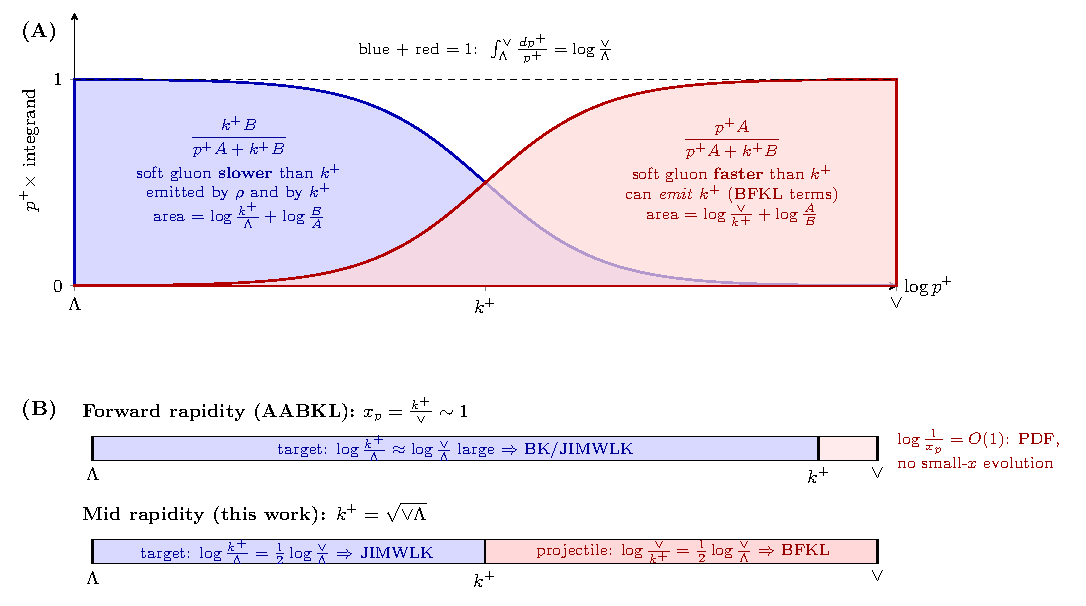
\includegraphics[width=\textwidth]{Origin_figure.pdf}
\caption{(A) The $p^+$ integrand of a row, times $p^+$, against $\log p^+$. The energy denominator splits it into a part at $p^+<k^+$ (blue: soft gluon slower, emitted by $\rho$ and by the measured gluon, target side) and a part at $p^+>k^+$ (red: soft gluon faster, can emit the measured gluon, projectile side). The areas are $\log\frac{k^+}{\Lambda}$ and $\log\frac{\vee}{k^+}$ (plus $\pm\log\frac AB$). (B) Forward rapidity: the projectile interval $\log\frac{1}{x_p}$ is $O(1)$, only the target evolves (AABKL). Mid rapidity: both intervals are $\frac12\log\frac\vee\Lambda$, both evolve.}
\label{fig:origin}
\end{figure}

%==========================================================================================
\section{Why this is not an interpretation: independence of the cutoffs}\label{sec:cutoff}
$\Lambda$ and $\vee$ are not physical. $\Lambda$ separates the soft gluons from the target fields; $\vee$ separates them from the valence charges $\rho$. The physical cross section cannot depend on where the two boundaries are put. At this order the dependence enters only through $\LT$ and $\LP$ in Eq.~\eqref{eq:LL}:
\begin{align}
-\Lambda\frac{\partial}{\partial\Lambda}\frac{d^3N}{d^3k}\bigg|_{\vee,k^+}&=\JJ=-H_{\rm JIMWLK}\,\frac{d^3N_{\rm LO}}{d^3k},\label{eq:dL}\\
\vee\frac{\partial}{\partial\vee}\frac{d^3N}{d^3k}\bigg|_{\Lambda,k^+}&=\JJ+(\BB-\JJ)=\BB={\rm LO}\Big[\langle\rho\rho\rangle\to K_{\rm BFKL}\otimes\langle\rho\rho\rangle\Big].\label{eq:dV}
\end{align}
\begin{itemize}
\item \textbf{Eq.~\eqref{eq:dL}.} Lowering $\Lambda$ moves gluons from the target into the soft window. To compensate, the target's Wilson-line distribution must change by $\JJ$. $\JJ$ is $-H_{\rm JIMWLK}$ acting on the Wilson lines of LO; the charges are untouched. This is the JIMWLK equation, here derived, not assumed.
\item \textbf{Eq.~\eqref{eq:dV}.} Raising $\vee$ moves charges from $\rho$ into the soft window. To compensate, the projectile's charge correlator must change by $\BB$. $\BB$ is LO with $\langle\rho^f(x)\rho^f(y)\rangle$ replaced by its coordinate-space BFKL evolution, and the Wilson lines are untouched. This is the BFKL equation.
\item \textbf{If the $\log\frac\vee\Lambda$ terms contained $\BB$}, Eq.~\eqref{eq:dL} would require a change of the target by $\JJ+\BB$. No change of the target Wilson lines can produce the 23 terms of $\BB$ in which the measured gluon is emitted by the soft gluon. So the structure of Eq.~\eqref{eq:LL} is forced.
\item \textbf{The same logic in AABKL.} They write: ``we do not have to specify what is exactly the evolution equation \dots\ This equation is self-consistently determined from the calculation itself'' (their Sec.~II.A). They then derive BK from $s_0\frac{d}{ds_0}\,d\sigma=0$ (their Eq.~(5.34)). Their $s_0$ is their target-side cutoff (Ioffe time), the analogue of our $\Lambda$, so this is Eq.~\eqref{eq:dL}.
\item \textbf{Wave-function picture} (\texttt{NLO\_gluon\_midrapidity.pdf}, Sec.~6). At leading log, the emissions are ordered in $p^+$, the harder first:
\begin{itemize}
\item for $p^+<k^+$, $\Omega=\Omega_p[\rho+j_k]\,\Omega_k[\rho]$: the soft gluon is emitted by $\rho$ and by the measured gluon. This gives JIMWLK;
\item for $p^+>k^+$, $\Omega=\Omega_k[\rho+j_p]\,\Omega_p[\rho]$: the measured gluon is emitted by $\rho$ and by the soft gluon. This gives BFKL.
\end{itemize}
\end{itemize}
At mid rapidity, $\LT=\LP=\frac12\log\frac\vee\Lambda$, so Eq.~\eqref{eq:LL} is $\frac12\log\frac\vee\Lambda(\JJ+\BB)$, the form of your corrected evolution file. Away from mid rapidity it is $\frac12\log\frac\vee\Lambda(\JJ+\BB)+\log\frac{k^+}{\sqrt{\vee\Lambda}}(\JJ-\BB)$.

%==========================================================================================
\section{Forward rapidity (AABKL) vs mid rapidity (this calculation)}\label{sec:aabkl}
\subsection{Setups}
\begin{itemize}
\item \textbf{AABKL} (T.~Altinoluk, N.~Armesto, G.~Beuf, A.~Kovner, M.~Lublinsky, arXiv:1411.2869): hybrid formalism.
\begin{itemize}
\item The projectile is a collinear proton (PDFs); the produced parton has large $x_p=p^+/P^+$.
\item LO is $\frac{1}{(2\pi)^2}x_pf(x_p)\int e^{ip(y-\bar y)}s_{Y_T}[y,\bar y]$, of order $\alpha_s^0$.
\item NLO is one extra gluon in the projectile parton's wave function.
\item The soft-gluon phase space is cut by an Ioffe-time condition, $\xi(1-\xi)x_pP^+/k_\perp^2>\tau$.
\end{itemize}
\item \textbf{This calculation:} the projectile is dilute valence charges $\rho$ with momentum $\vee$.
\begin{itemize}
\item LO is the gluon radiated by $\rho$ (Kovchegov--Tuchin type), of order $\alpha_s$, with $\langle\rho\rho\rangle$ and the trace ${\rm Tr}\{(U^\dagger(x)-U^\dagger(y))(U(x')-U(y'))\}$.
\item NLO is one extra gluon in the window $\Lambda<p^+<\vee$, with sharp cutoffs.
\end{itemize}
\end{itemize}

\subsection{Rapidity intervals and evolution}
\begin{itemize}
\item AABKL, Sec.~II.A: ``the projectile wave function at any energy is evolved only to rapidity $Y_p=\ln\frac{1}{x_p}+Y_0$''; the target is evolved by $Y_T$ (their Eq.~(2.11), Fig.~1).
\begin{itemize}
\item With $x_p\leftrightarrow\frac{k^+}{\vee}$: $\ln\frac1{x_p}=\LP$, and $Y_T$ plays the role of $\LT$.
\item This is the split of Eq.~\eqref{eq:LL}.
\end{itemize}
\item They derive the energy dependence at \emph{fixed} $x_p$ (their Eq.~(5.32): ``production at fixed $x_p$ but at higher energy''). At fixed $a=\frac{k^+}{\vee}$, $\LP=\log\frac1a$ is constant and Eq.~\eqref{eq:LL} gives $\frac{d}{d\log\vee}\,\frac{d^3N}{d^3k}=\JJ$: only the target evolves. This is their BK result. Their Eq.~(5.39) is the same evolution acting on a fundamental dipole, i.e.\ the quark channel.
\item They neglect the $P^+$ dependence of the projectile distribution because $x_p$ is not small. In their words (Sec.~III.A, item 3): ``For small values of $x$ one indeed has to take into account the $P^+$ dependence''.
\begin{itemize}
\item At mid rapidity $x_p=\frac{k^+}{\vee}=\sqrt{\Lambda/\vee}$ is small and $\LP=\frac12\log\frac\vee\Lambda$ is as large as the target interval.
\item That $P^+$ (i.e.\ $\vee$) dependence is our Eq.~\eqref{eq:dV}: the BFKL evolution of the projectile.
\end{itemize}
\item \textbf{So at leading log, the forward limit of our result is AABKL's structure.} The one difference at mid rapidity is that the projectile interval is large and must be resummed.
\end{itemize}

\subsection{Term by term}
{\small\renewcommand{\arraystretch}{1.25}
\begin{longtable}{@{}>{\raggedright\arraybackslash}p{0.27\textwidth}>{\raggedright\arraybackslash}p{0.27\textwidth}>{\raggedright\arraybackslash}p{0.1\textwidth}>{\raggedright\arraybackslash}p{0.28\textwidth}@{}}\toprule
AABKL (forward), Eqs.~(4.20)--(4.22) & this work (mid rapidity), \texttt{Finite\_terms\_singlet.pdf} Eq.~(7.1) & & comment\\\midrule\endhead
target evolution: BK for $s_{Y_T}$, from $s_0$-independence & $\LT\,\JJ$ (JIMWLK), from $\Lambda$-independence & same & same kernel; BK is the large-$N_c$ dipole form\\
projectile: PDF $f(x_p)$, no small-$x$ evolution & $\LP\,\BB$ (BFKL of $\langle\rho\rho\rangle$) & different & $\LP=\ln\frac1{x_p}$ is $O(1)$ forward, $\frac12\log\frac\vee\Lambda$ at mid rapidity\\
LO: $x_pf(x_p)\,s_{Y_T}[y,\bar y]$, $O(\alpha_s^0)$ & LO: WW gluon of $\rho$, $O(\alpha_s)$, ${\rm Tr}\{(U^\dagger(x)-U^\dagger(y))(U(x')-U(y'))\}$ & different & collinear parton vs.\ $k_\perp$-dependent emission by colour charges\\
hadron convolution $\int_{x_F}^1\frac{d\zeta}{\zeta^2}D(\zeta)\dots$ & $\int_{k^+/\vee}^1\frac{d\zeta}{\zeta^2}D_{h/g}(\zeta)\dots$ & same & lower limit from the largest projectile momentum\\
fragmentation (after-target) term, $P_{gg}$ with $[\cdot]_+$, $\int_0^{1-x_p}d\xi$ & DGLAP term, $-\frac{\alpha_s}{2\pi}\int_{a}^1\frac{d\xi}{\xi^2}P^{(r)}_{gg,+}{\rm LO}_\xi[\ell_\Delta]$ & same & same splitting function, plus prescription and limit; $f_{\mu^2}=f^{\overline{MS}}_{1.26\mu^2}$ is our $c_0^2=1.26$\\
PDF (before-target) collinear term & G2 Row I part 2: finite & different & our parent is emitted at distance $|x-w|$ from a charge; no collinear pole, no PDF\\
interference and virtual colour structures ($sss$, $\overline X/N_c^2$) & ${\rm Tr}\{T^eAT^eB\}$ traces of Secs.~5, 6 & same colour & kinematics differ (emission by charges, energy denominators $p^+A+k^+B$)\\
virtual term, $\int_0^1d\xi$ (no $x_p$ limit) & G1 Row II: limit $\xi\ge\frac{k^+}{\vee}$ $\Rightarrow$ $V_\vee$ and the Q1 pole & different & with AABKL's choice both disappear\\
soft gluon cut by the Ioffe time; ``evolution interval'' depends on $l_\perp$ (their Eq.~(3.13)) & sharp cutoffs $\Lambda<p^+<\vee$ & scheme & changes $O(\alpha_s)$ finite terms, not the logarithms\\
--- & running coupling of the LO $g^2$; CMW constant $\frac{67}{9}-\frac{\pi^2}{3}$ & only here & AABKL's LO has no coupling to renormalize\\
--- & linear polarization term & only here & our incoming gluon is the polarized WW field\\
--- & the LO (parent) gluon emitted after the target by the rotated charge & only here & charges, not a parton, radiate; AABKL's parent parton exists before the target\\
--- & three- and four-$\rho$ terms & only here & several charges; zero or Gaussian-reducible for a Gaussian projectile\\
quark channels ($C_F$ terms, Eq.~(4.21)) & --- & only there & $n_f=0$, no quarks in our projectile\\\bottomrule
\end{longtable}}

\subsection{Verdict}
\begin{itemize}
\item \textbf{``Mostly the same'' holds for:} the target evolution, the final-state (fragmentation) side, the hadron convolution, and the colour structures of the one-gluon real and virtual terms. These are the parts that do not depend on what the projectile is.
\item \textbf{It does not hold for the projectile side}, because the two LOs are different objects: a collinear parton with a PDF vs.\ a gluon radiated by colour charges. This difference is not a small correction:
\begin{itemize}
\item at mid rapidity there is a second large logarithm, $\log\frac{\vee}{k^+}$, with BFKL;
\item there are the running coupling of LO, the linear polarization, emission after the target, and the multi-charge terms;
\item there is no PDF DGLAP.
\end{itemize}
\item \textbf{The finite constants are scheme dependent} (Ioffe time vs.\ sharp cutoffs). A term-by-term numerical agreement of the finite parts is not expected even where the structures match.
\item \textbf{Consistency check that does hold:} at leading log, our Eq.~\eqref{eq:LL} at fixed $k^+/\vee$ reproduces AABKL's evolution structure: target only, interval set by the produced particle, nothing for the projectile.
\end{itemize}
\end{document}
